%!TEX root =  main.tex
%\appendix
\chapter{Detailed List of Self-Healing Approaches}
\label{ap:approches}
This appendix report describes the different self-healing approaches which has been used by authors  \ldots 

\section{Brun's self-adapting reliability} \label{ap:BurnSelf}
\begin{compactitem}
\item[\textbf{Title}]Self-Adapting Reliability in Distributed Software Systems
\item[\textbf{Author}] 
Yuriy Brun, Jae young Bang, George Edwards and Nenad Medvidovic
\item[\textbf{Reference}] 
\cite{brun_self-adapting_2015}
\item[\textbf{Year}] 
2015
\item[\textbf{Application Domain}] 
Distributed computation architecture
\item[\textbf{Self-Healing steps}] Self-healing steps involved are fault-detecting, diagnosis and recovering
\item[\textbf{Technical Approach}]Iterative redundancy technique
\item[\textbf{Basic Idea}] 
The iterative redundancy algorithm aims to deploy the minimum number of jobs to get a consensus in a correct result. If this does not happen, it iteratively deploys the minimum number of additional jobs until a consensus is reached. 

\item[\textbf{Summary of approach}]
Distributed computing architectures ensure the correct execution of each task through voting: multiple independent computational nodes perform the same task and if the majority of executions agree on a result, a consensus exists, and that result is taken to be the solution of that task. Iterative redundancy tries to optimize the use of computational nodes by distributing the minimum number of jobs that perform the same task required to achieve a desired confidence level in the result, assuming that all the jobs’ results agree. Then, if all jobs agree, the task is completed. However, if some results disagree, the confidence level associated with the majority result is diminished because of the chance that the disagreeing results are correct. The proposed approach then reevaluates the situation and distributes the minimum number of additional jobs that would achieve the desired level of confidence. This process repeats until the agreeing results sufficiently outnumber the disagreeing results to reach the confidence threshold. The flow digram of the algorithm is given by:

\begin{figure}[H]
\center
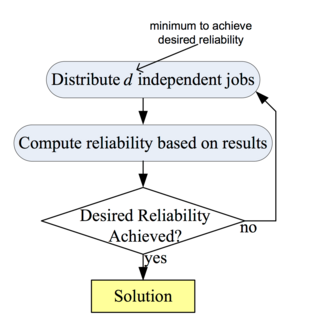
\includegraphics[width=5in]{img/Iterativeredundancyschematic}
\caption{Flowchart of Iterative Redundancy Algorithm}
\end{figure}


\item[\textbf{Fault Types}]Byzantine attacks: A Byzantine fault is one where the faulty unit continues to run but produces incorrect results and might lead to failure sometimes. 

\item[\textbf{Failure Types}]Functional failures.

\item[\textbf{Input data}] Results produced by n independent jobs that perform the same task.

\item[\textbf{Recovery actions}]The technique try to  iteratively deploy the minimum number of redundant jobs in order to achieve a consensus on a correct result.

\item[\textbf{Advantages}] Iterative redundancy is more cost effective, than traditional redundancy approaches as it creates the same level of software system reliability at a lower expense.

\item[\textbf{Disadvantages}] In iterative redundancy, the task server deploys several jobs and wait for the responses before possibly choosing to deploy more jobs. Therefore, this technique increases the latency for a particular task.

\item[\textbf{Case studies}]
The technique is implemented and tested on PlanetLab. PlanetLab is a gathering of PCs accessible as a testbed for distributed systems research.\\
\end{compactitem}


\section{SHoWA} \label{ap:Showa}
\begin{compactitem}
\item[\textbf{Title}]A Self-Healing Framework for Web-Based Applications (SH\~oWA)

\item[\textbf{Author}]Joao Paulo Magalhaes and Luis Moura Silva

\item[\textbf{Reference}]

\cite{magalhaes_showa:_2015}

\item[\textbf{Year}] 2015

\item[\textbf{Application Domain}]
Web-based applications. 

\item[\textbf{Self-Healing steps}] 
The self-healing steps involved are:Monitor, Plan, Analyse and Execute.

\item[\textbf{Technical Approach}] Statistical correlation (Spearman's rank correlation). 
%The Spearman's rank correlation coefficient (rho) measures the statistical dependence between two variables.

\item[\textbf{Basic Idea}] 
The basic idea is to collect and analyse system, application server, and application-level data, such as response time of user transactions and amount of available memory, so as to detect and pinpoint anomalies by means of statistical correlation. The performed data analysis detects changes in the server response time and analyses if those changes are correlated with a workload variation or are due to a performance anomaly. In the presence of performance anomalies, the analysis pinpoints the method calls that are more likely responsible to cause the anomaly.

\item[\textbf{Summary of approaches}] 

SH˜oWA FRAMEWORK

The SH\~oWA framework mainly works in four steps: Monitor, Analyse, Plan, and Execute. The monitor steps is executed by the sensor and data interpretation module. The analyse step is executed by the workload variation analysis, performance anomaly analysis, anomaly detector and root-clause failure analysis module. The plan step is executed by the recovery planner module and the execute step is executed by the executor and effector module. The digram below shows the different modules of the  SH\~oWA framework.

\begin{figure}[H]
\center
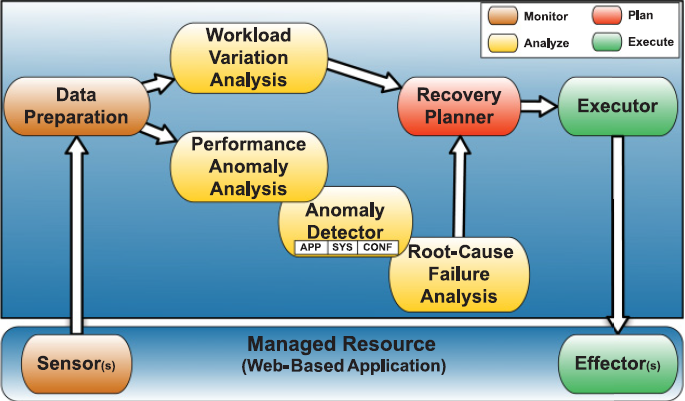
\includegraphics[width=5in]{img/selfhealingframework}
\caption{(SH\~oWA).: self healing framework}
\end{figure}

The Sensor module collects data from different system and application server parameters and measures the execution time of user transactions and application calls. The data is sent to a remote database to be prepared by the Data Preparation module. The Workload Variation Analysis and Performance Anomaly Analysis modules carry out statistical analysis to detect response time variations and to verify if the response time variations are due to workload changes or are a symptom of a performance anomaly. The Anomaly Detector module carries out statistical analysis to detect if there is any change in the system or application server parameters correlated with the performance anomaly. The Root-cause Failure Analysis module carries out statistical analysis to analyse the response time of the application calls to check if there are changes in the application, or in the invocation of remote services, that are correlated with the performance anomaly. Upon the detection and localization of performance anomalies, the recovery phase follows. The recovery phase involves the Recovery Planner module, which is responsible for selecting the recovery procedure, and the Executor module, which dispatches the recovery actions to be applied on the managed resource by the Effector module.\\

The sensor module monitors key performance indicators such as CPU load, JVM heap memory, number of open files and number of running threads. Additionally, it gathers execution time of application transactions. The data collected by the sensor module is processed by the data preparation module that associates each measurement to a specific user transactions of the monitored web application. The prepared data is then passed to the workload variation analysis and performance anomaly analysis modules to detect and pinpoint if any anomaly is present. The data analysis is based on Spearman's rank correlation coefficient represented by rho ($\rho$). The correlation coefficient is given by the equation below and  expresses how two variables are associated:

%begin{figure}[H]
%includegraphics[width=5in]{img/formulae}
%caption{Measure of statistical dependence between two %variables.}
%end{figure} 

%\rho=\frac { \sum_{ i=1} ^n(X_i-\bar{ X})(Y_i-\bar{ Y})}%%%{\sqrt{\sum_{ i=1} ^n (X_i-\bar{ X})^2 (Y_i-\bar{ Y})^2} }
%}

\begin{equation}
\rho=\frac { \sum_{ i=1} ^n(X_i-\bar{ X})(Y_i-\bar{ Y})}{\sqrt{\sum_{ i=1} ^n (X_i-\bar{ X})^2 (Y_i-\bar{ Y})^2}}
\end{equation}


where X is the sequence of the accumulated response server time per user transaction and Y is the number of user transactions processed in the same interval.If p remains stable and high across the periods of analysis, then it means that the response time is associated with the application workload (e.g., bursty workload, server queue issues). If p  decreases, then it means that one of the variables has increased or decreased while the other has remained stable or changed in an opposite direction. This dissociation corresponds to a symptom of performance anomaly (e.g. performance slowdowns from the number of user transactions processed.).Once the performance anomaly is identified by using  Spearman's rank correlation coefficient, the anomaly detector module aims to identify if there is a system or application server changes which is associated with the performance anomaly. As in the previous analyses, the anomaly detector module computes Spearman’s rank correlation coefficient $\rho$ between  the total number of user transactions processed in an interval and the accumulated value of the parameters collected by the Sensor module in the same interval. If the accumulated value of a given parameter increases and is not motivated by an increase in the number of user transactions, then the $\rho$ degree will decrease, showing that a parameter is no longer aligned with the number of requests and associating this with the performance anomaly. The data analysis in this module determines if the application is facing a performance anomaly and verifies if the anomaly is associated with changes in the parameters. If the performance anomaly is confirmed by the anomaly detection module, the root cause analysis module analyses user transactions that have only reported a performance anomaly in the previous stage. 
The root cause failure analyses module analyses the frequency of the response time of a user transaction and the response time frequency for the calls belonging to the user transaction under analysis. By applying the Spearman’s correlation analysis,this module is able to determine the list of method calls associated with the performance anomaly.

%In the current implementation, the recovery actions are procedure based and defined by human operator.In future research prospect, it is a novel idea to design the recovery procedures using the machine learning techniques.Once selected, a recovery procedure is executed by the executor module. The main job of the executor module is to execute the specific recovery action which has been triggered with respect to the specific anomaly detected.Once the recovery action has been executed, the handler is passed to the effector module which monitors and keeps track of the number of call methods that has triggered anomaly, how many
%of these are in recovery and how any of them has already been recovered.In future research prospect, it is a novel idea to design the recovery procedures using the machine learning techniques.

\item[\textbf{Fault types}]Fail-stutter fault model. 

In fail-stutter fault model, the components of a system sometimes fail and sometimes perform erratically (e.g., low performance) but are not reflected in the final results. These unexpected behaviors are defined as performance faults.

\item[\textbf{Failures types}]Performance failures.

\item[\textbf{Input data}] The input are the parameters which are collected by the sensor module. For instance user transactions, CPU time per user transactions, amount of available memory.

\item[\textbf{Recovery actions}]The output are the recovery strategies which are carried forward or executed against the particular anomalies detected.

\item[\textbf{Advantages}] In SH\~oWA sensor module the monitoring code is separated from the application code, thereby an application can be monitored without the need for manually changing its source code. With this separation, multiple applications can be monitored using the same monitoring code. The framework is generic and can be applied to any type of transactional web application. The only module that needs to be ported is the Sensor module

\item[\textbf{Disadvantages}]The ability to detect anomalies while the number of end users affected is low.
We need the source code of the application to deploy the sensor module.

\item[\textbf{Case studies}]One retail store web application and an auction web application has been used in this paper for testing the framework.
\end{compactitem}


\section{GenProg}\label{ap:GenProg}
\begin{compactitem}
\item[\textbf{Title}]GenProg: A Generic Method for Automatic Software Repair

\item[\textbf{Author}]
Claire Le Goues, ThanhVu Nguyen, Stephanie Forrest, and Westley Weimer

\item[\textbf{Reference}]  

\cite{le_goues_genprog:_2012}

\item[\textbf{Application Domain}]
Web application 

\item[\textbf{Self-Healing steps:}]. The closed loop repair system works in this way. The method adopts an IDS (intrusion-detection system) that detects the anomalies in the system. Whenever, the IDS detects an annomaly, GenProg is invoked to repair the suspicious behavior.

\item [\textbf{Technical Approach}] 

The technical approach used in this paper is genetic programming. Genetic programming (GP) is an evolutionary algorithm-based methodology which uses a set of instructions and a fitness function to measure how well a computer has performed a task.

\item[\textbf{Basic Idea}]

The basic idea is that the IDS detects an anomaly in the request and if there is an anomaly then there is an attack  and the system is stopped. Then the GenProg is invoked which takes input of the negative test case, positive test cases, and the defect and generates a variant. The variant is the automatic recovery which contains the program requirement. The variant which has the highest fitness function is considered to be the best.

A negative test case is a test case which contains the bug, if there exists a bug.

genetic program repair technique "GenProg", which uses existing test cases to automatically generate repairs.The GenProg takes an input of the set of positive test cases and the defect, searches for a program variant which retains the functionality, evaluates each variant with a user-defined fitness function and individuals with high fitness are selected for continued evolution.The variant which passes all the test cases are taken into consideration for generating the automatic final repair.

\item[\textbf{Summary of approach}] The approach implements three functions: The \textit{initialpopulation} generates the variants by using the mutual operators based on the input program and test cases. The \textit{fitness function} evaluates each variants created and chooses the best amongst them and the \textit{GenProg} iterates by selecting high fitness individuals, which are selected for continuous evolutions for the next.


The technical approach used in this paper by the author can be classified in four stages:-
\textit{Program Representation:}Each variant is represented by a pair of an abstract syntax tree   (AST)and a weighted path. The abstract syntax tree contains all the statements of the program and a weighted path contains all the statements in the program that has been assigned a weight based on the occurrence of the statement the test cases.\textit{Selection and Genetic Operators:}genProg discards individuals with fitness 0 (variants that do not compile or that pass no test cases) and places the remainder in Viable. It then uses a selection strategy to select pop size/2 members of a new generation from the previous iteration.\textit{Fitness function:}the fitness function evaluates the acceptability of a program variant. The fitness function mentioned in this paper, encodes software requirements at the test case level: negative test cases encode the fault to be repaired, while positive test cases encode functionality that cannot be sacrificed.\textit{Repair Minimization:}
the search terminates successfully when GP discovers a primary repair that passes all test cases. Due to randomness in the mutation and crossover algorithms, the primary repair typically contains at least an order-of-magnitude more changes than are necessary to repair the program, rendering the repairs difficult to inspect for correctness.


\item[\textbf{Fault Types}]Infinite loop, Segmentation fault, Remote heap buffer over flow to inject code, Remote heap buffer overflow to overwrite variables, Non overflow denial of service, Local stack buffer overflow, Integer overflow and Format string vulnerability.

\item[\textbf{Input data}] Input source code contains a failing negative test case that exercises the defect and a set of passing positive test cases that describe requirements.

\item[\textbf{Recovery actions}]The recovery action is the primary repair that passes all test cases.

\item[\textbf{Advantages}] 
The GP search space focuses genetic operations along a weighted path and takes advantage of test case coverage information, and reusing existing program statements.

\item[\textbf{Disadvantages}] GenProg relies on test cases to encode both an error to repair and important functionality. GenProg cannot repair race conditions as it is difficult to encode an error using test cases for non-deterministic properties.

\end{compactitem}

\section{QVM}\label{QVM}
\begin{compactitem}

\item[\textbf{Title}]QVM: An Efficient Runtime for Detecting Defects in Deployed Systems

\item[\textbf{Author}]
Mathew Arnold, Martin Vechev and Eran Yahav

\item[\textbf{Reference}] 

\cite{mathew_arnold_qvm:_2008}

\item[\textbf{Year}] 2011

\item[\textbf{Application Domain}] Java application


\item[\textbf{Self-Healing steps}] Self-healing steps involved the following:

(i)	Finding Bugs.
The QVM monitors the correctness properties and resource leakage. The report for the bug includes the information about the allocation of the object, the object’s last state and the method invoking the object.

(ii) Diagnosing the Cause.
The QVM provides debug information in form of type state history. For every invocation, the invocation history collects the information about the context in which the object was invoked. Hence, with the object-centric sampling, the detailed debug information is collected with low overhead.

(iii)	Developing a Fix.
QVM heap assertion leverages and checks the object for its sharing. This is done in the testing phase for fixing the problem and removal before the deployment. The problem is healed up with repetitive application of the method until the reported leak does not occur.    

\item[\textbf{Technical Approach}]

The QVM extends the VM execution engine with three main components: 
(i)	QVM interface
(ii)Overhead Manager and
(iii)QVM Clients 

\item[\textbf{Basic Idea}]  

The study is on the usability of interactive applications running with QVM. The QVM detects defects by continuously monitoring the execution of the application by checking typestate safety properties, Java assertions, and heap properties pertaining to ownership. It also provides a balanced trade-off between the cost of the monitoring process and the maintenance of sufficient accuracy for detecting defects.

\item[\textbf{Summary of approach}] Quality Virtual Machine (QVM) is a runtime environment that uses the technology and infrastructure available in a virtual machine (VM) to improve the software quality. It provides an interface that allows software monitoring clients to be executed in a controlled overhead. The goal of the system is to provide a solution having performance with low overhead and to provide maximal separation of the clients from the underlying architecture. The QVM is three tier architecture having clients at the abstract level, QVM Interface as the middleware bridging the gap among the clients and QVM’s working at the core. The input to the QVM is a user-defined overhead estimation value and the bug log report. At the initial stage the application program is connected with the QVM clients that play a major role for evaluating the performance of the system. The type state, heap probes and assertions the major clients of QVM that generate the violation report for the QVM. 

The QVM Interface (QVMI) performs three different tasks as 
1. Filtering. Filtering is done for addressing the callback requests irrespective of the working of the system. The VM provides dynamic optimization techniques to achieve an efficient implementation of the sampled profile.

2.	Property Guided Sampling. Sampling is a key mechanism for QVM that reduces the overhead. It provides dynamic analysis of the objects with its associate’s properties. With the typestate properties, the relation between the events for same object needs to be maintained.

3.	Object Centric Sampling.     At the object instances level, the objects are tracked with profile events with the objects. The tracking of objects is done at allocation time. The object sampling produces meaningful results without destroying properties associated with objects.

The OverHead Manager (OHM) known as the core of the system does the estimation of the overhead by specifying the overhead budget 5-10 \% of the deployed system. For a given overhead budget, the QVM accumulates much of information about the object. The information gathering is done by three strategies. (i)	Monitoring. Monitoring is done by assigning a timer to the QVMI entry, exist calls and time spent on the clients. For this the QVM deploys accurate timers so that time working and existing of the threads can be tracked properly.

(ii) Sampling. With the Sampling method QVM maintains a log for each event. A sample counter and sampleCounter Reset are added to the code for keeping the track of the event execution and abort. For severe performance degradation the QVM supports the notion of an emergency shutdown.

(iii)	Controlling. The Overhead Controller checks the QVM overhead and adjusts the sampling frequencies. The frequencies are adjusted as the budget increases or decreases periodically. Even a overhead beyond the budget can cause an emergency shutdown.
However, with early tracking of the objects, early resource release can be done for increasing the performance. 

\begin{figure}[H]
\center
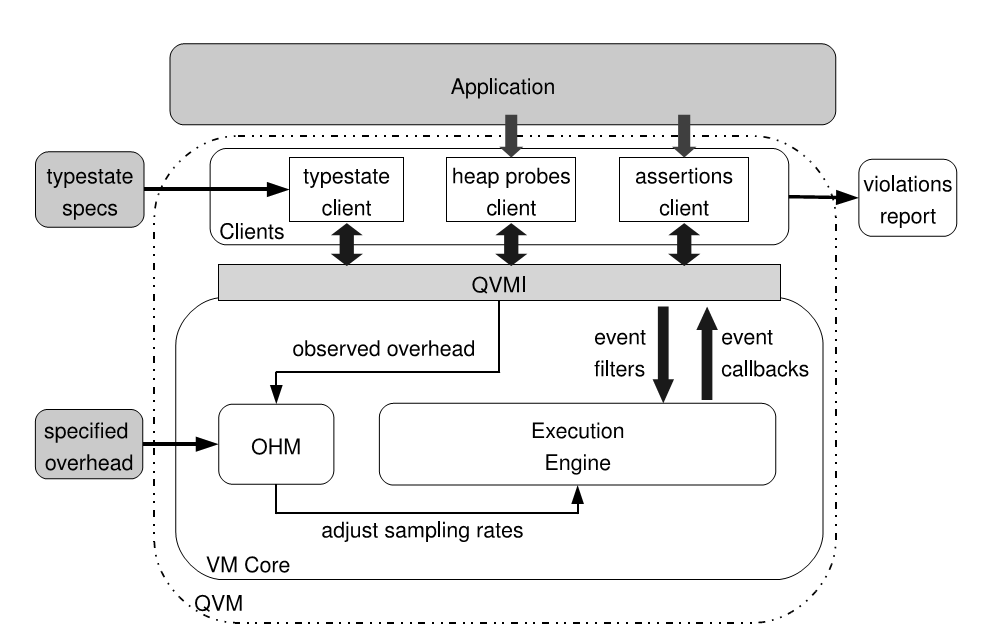
\includegraphics[width=5in]{img/qvm}
\caption{Overall architecture of QVM.}
\end{figure}

\item[\textbf{Fault Types}]
(i)	    Typestates assertions
(ii)	Resource Leakage
(iii)	Java assertions
 
\item[\textbf{Failure Types}]

(i)	Performance Degradation

\item[\textbf{Input data}] 

(ii)	Overhead estimation
(iii)	Bug log file


\item[\textbf{Recovery actions}]

(i)	Resource utilization
(ii)Leverage heap probe 


\item[\textbf{Advantages}] 

(i)	High-performance and low overhead
(ii)	Maximal separation of analysis clients from virtual machine (VM)
(iii)	Runtime access for the clients allows for utilizing information
(iv)	The access to dynamic optimizer (JIT) ensures to critical code paths are well optimized
(v)	The efficient dynamic updating of VM can be upgraded with the application of the advance techniques such as code patching and on-stack replacement.  
(vi)	The deployment becomes easier as the required features are installed in the VM.


\item[\textbf{Disadvantages}] 

(i)	    Quality service implementation on VM makes them non-portable
(ii)	The users of the system are meant specific to VM version

\item[\textbf{Case study}] 

(i)	Azerus- A bit torrent client protocol.
(ii) etrader (trading platform) (iii) feednread (newsfeed reader) (iv) goin (IM client) (v) ibm app1 (large scale product) (vi) ibm app2 (medium scale tool) (vii) jcommander (file manager) (viii) juploader (flickr upload tool) (ix) nomadpim (personal information manager) (x) rssowl (rss news reader) (xi) tvbrowser (tv program guide) (xii) tvla (program analysis framework) (xiii) virgoftp (FTP client). 

\end{compactitem}
\section{MAPE-K}\label{MAPE-K}
\begin{compactitem}

\item[\textbf{Title}]MAPE-K Formal Templates to Rigorously Design Behaviors for Self-Adaptive Systems

\item[\textbf{Author}]Didac Gil De La Iglesia, Danny Weyns

\item[\textbf{Reference}] 

\cite{didac_iglesia_mape-k:_2015}

\item[\textbf{Year}] 2015

\item[\textbf{Application Domain}]Distributed Systems 

Self Adaptive systems that are worked as example are

(i) Mobile learning (ii) Robotics

\item[\textbf{Self-Healing steps}] Self-healing steps   involved the following:

(i) Monitor (ii) Analyze (iii) Plan (iv) Execute 
(v) With Knowledge

\item[\textbf{Technical Approach}]
The MAPE-K template is deployed in the system comprise the behaviour specification templates and property specification template specifying the property behaviours formal verification.

(i) Behaviour specification templates- Timed Automata

(ii) Property specification template – Timed Computational Tree Logic

\item[\textbf{Basic Idea}]  
The basic idea is to develop a self adaptive system that would deal with the concerned domain and adapt to the structure and modify their behaviour at run time with little or no human intervention. This will heal the managed system when a fault is detected.


\item[\textbf{Summary of approach}] In the dynamically changing system, prediction of availability of resources and detection of fault has become difficult. To address the problem self-adaptive systems are developed. The self-adaptive systems can reconfigure their structure and modify their behaviour at runtime with a little or no human intervention. The system consists of a managed system and a feedback loop. The managed system deals with the concerned domain users and feedback loop deals with adaptation of the managed system.

The feedback loop consists of five phases together known as MAPE-K as: (1) Knowledge (2) Monitor (3) Analyze (4) Plan (5) Execute

The MAPE-K template comprises of

(i) Behavioural Specification template for modelling different components of MAPE-K and their interactions. The Timed Automata (TA) with clock variable for state and transition between the states representing actions is deployed.

(ii) Property Specification template for specifying required properties of the adaptation behaviours enabling formal verification of the behaviours. A Timed Computational Tree Logic (TCTL) is deployed with extended clock variable that allows specification of properties such as reachability, liveness and safety.With the distributed self-adaptive system multiple local managed systems are deployed at nodes and have MAPE-K feedback loops. The basic focus of the self-adaptation deals with robustness and openness of the system that is, addition and deletion of resources can be done as required and self-healing is done when system failure occurs. To elaborate the MAPE-K feedback loop a Mobile Learning System application is explained where the application is to learn the geometry concepts with GPS enabled mobile devices. The basic resources in this domain are GPS services.

The MAPE-K feedback loop is detailed as follows:

(i) Knowledge- Each component in the MAPE is dependent on the knowledge of the system. The knowledge of the system has four categories. 

a. Managed System Knowledge- this part of knowledge comprises of the system knowledge as number of nodes, number of resources, type of resources, and quality of resources. 

b. Environment Knowledge- the knowledge is about the environment of domain where the system is deployed.

c. Concern Knowledge- the knowledge is to realize the requirement of resources to fulfil the goals of self adaptive systems.

d. Adaptation Knowledge- the knowledge to represent the working and behaviour of the system. The indirection synchronization of behaviour is flagged by the system.(ii) Monitor

Monitor collects the data through searching from the managed system and the environment to update Knowledge. Before updating the pre-processing is done with methods such as normalization, filtering and aggregation. The monitor performs the task of identifying the failure and resource request and updating the knowledge for analyzing 
the behaviour. Hence the monitor behaviour performs triggering, collecting the related information, pre-processing the data, working data, and call to analyze.

(iii) Analyze

Analyze is done to determine is the adaptation actions required based on the information from the monitor and the environment of the system. The Analyze behaviour has three 
primary states: 

a. Satisfied- the managed system has sufficient number of resources it requires to achieve the goal. 

b. Under-satisfied- the system lacks the resources for achieving the goal.

c. Over-satisfied- the system has redundant number of resources.

Hence, the Analyze phase performs the triggering, data collection, analysis and call to Plan phase.(iv) Plan

The planning mitigates actions to adapt the managed system when the resources are required. Depending on the analyze phase the planning is done. No adaptation plan is required when system is satisfied. The resources need to be added when the system is underestimated. The resources are to be released when the system is over satisfied.(v) Execute
The Execute behaviour is responsible for executing the adaptation actions of the generated plans. If the system is not ready, the behaviour performs the preparation task 
before executing the actions for addition of the resources to the system. The preparation tasks include locking of certain resources keeping the system in safe state. After the execution is complete, the plan is checked for its completion. If some actions remain pending, the process is repeated for next actions to the managed system.Apart from the behavioural specifications, the Property verification templates are added to the system with the help of TCTL. The template has three groups as:

(i) Adaptation Goal specification- properties related to realization of adaptation goals by MAPE-K feedback loop. (ii) Intra-Behaviour Specification Template-specifies properties of internal MAPE component behaviour. (iii) Intre-Behaviour Specification Template-specifies properties for interaction between multiple behaviour of MAPE-K loop.

\begin{figure}[H]
\center
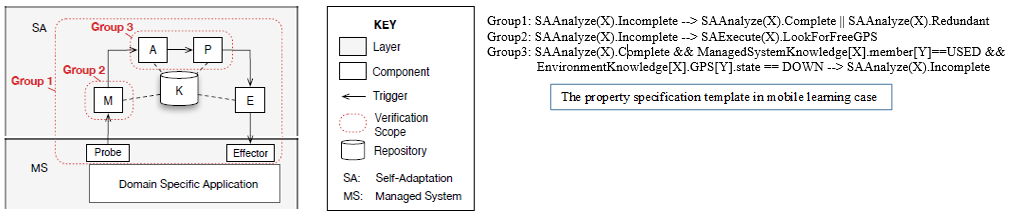
\includegraphics[width=5in]{img/pst}
\caption{Groups of property specification template.}
\end{figure}

\item[\textbf{Fault Types}]
(i) System breakdown (ii) System deadlock
\item[\textbf{Failure Types}]

Failure Types (i) Shortage of resources
\item[\textbf{Input data}] 
(i) Nodes- Number of nodes (ii) NRes-Number of resources
(iii) availableResources[NRes]- number of available resources


\item[\textbf{Recovery actions}]
The plan and execute phase performs the task of recovery as MAPE performs the post execution tasks with the postAction () function. The requirement of resources or release of resources changes the environment of the system. With PostExecutionAdd() function the required resources are added to the system. If more actions are Pending the system checks for PrepareAdd state and repeats the process to execute the actions so the system does not waits for and can recover from shortage of resources, making the resources available.


\item[\textbf{Advantages}] 
(i) Self-adaptive systems deals openness- the system can add and delete resources such as nodes, subsystems and components as required.
(ii) The self-healing process recovers from the system failure.

\item[\textbf{Disadvantages}] 
(i) The Timed Automata (TA) is modelling language supporting modelling for behavioural aspects of design. Therefore to model the message and communication protocols used in distributed systems can be difficult to model with the language of primitives of timed-automata.

\item[\textbf{Case study}] 
(i) Smart homes (ii) Security system (iii) Vehicular traffic systems

\end{compactitem}
\section{Azim's selfhealing smartphone software}\label{AzimSelf}
\begin{compactitem}
\item[\textbf{Title}] Towards Self-healing Smartphone Software via Automated Patching
\item[\textbf{Author}]
Tanzirul Azim, Iulian Neamtiu and Lisa Marvel\item[\textbf{Reference}] 

\cite{tanzirul_azim_smartphone:_2014}

\item[\textbf{Year}] 2014

\item[\textbf{Application Domain}]
Mobile applications for an android device

\item[\textbf{Self-Healing steps}] Self-healing steps involved are monitoring, detecting and recovering.

\item[\textbf{Technical Approach}]

Static analysis, dynamic analysis and bytecode rewriting

\item[\textbf{Basic Idea}]  
In this paper the basic idea is to introduce a methodology that uses automatic error detection and patch development towards giving a self-healing abilities to android applications. The author utilizes dynamic analysis to identify crash points, static analysis to recognize rollback points, and binary rewriting to seal of routines associated with crash points so that applications can keep on working even after an accident, with restricted functionality. The author tested the framework in detecting and fixing bugs in several popular android apps for instance facebook mobile, NPR news and K-9 mail. 

\item[\textbf{Summary of approach}] 
The summary of approach is summarised below:

\begin{figure}[H]
\center
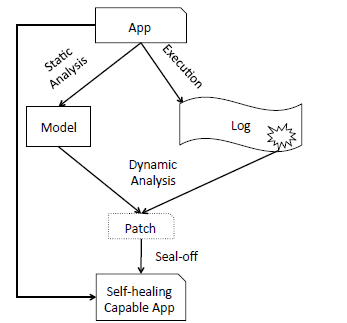
\includegraphics[width=5in]{img/smartphone_2014}
\caption{System architecture}
\end{figure}

(i)Model construction and roll-back point identification. First, the author derives a model (State activity transition graph) from the app via static analysis on the app bytecode, where nodes represents GUI app screen and edges represents transition between screens. The SATG graph is constructed with an open-source tool Automatic Android App Explorer (A3E), which is used for systematically exploring android applications running on phone. A3E supports sensors and does not require access to source code. The A3E keeps a track of monitoring, profiling, information flow tracking of the application. The graph identifies the rollback points (safe and unsafe points in the app). Safe points will be roll-backed and unsafe points will be sealed off. The model includes rollback (resume) points where the app will be driven when recovering from a fault.

(ii)Detection. Second, when the app is executed the Android Dalvik virtual machine constantly monitors the app via dynamic analysis and when a fault occurs the VM reports the potential cause of the error and the associated method with the fault in the log file. To implement monitoring, the author adds a sensor module, listener in the Dalvik VM's logging system. After analysing the log, VM finds that the closest method associated with the crash. This concludes the online fault detection phase. 

(iii)Recovery. Once a failure is detected the application rollbacks and resume the app. The rollback point depends on whether the fault is transient or persistent. In case of transient fault (temporary error, viz. network failures) the rollback point is the same point where the crash has been encountered. In case of persistent fault (permanent error, viz. unhandled exception), a patch is created to seal of the functionality which is responsible for the crash. The patch is created via dynamic analysis and in this case the rollback is the earlier node in the SATG and the author uses bytecode rewriting to seal of the faulty method in the faulty SATG node. Bytecode rewriting was done by the author using the smali Dalvik assembler/disassembler. In both types of faults, the author used the systematic exploration component of A3E, to drive the execution, so we could reliably drive the app into a state where it crashes.

\item[\textbf{Fault Types}]

Transient and persistent faults
(i)Transient faults are temporary faults such as unexpected shared memory deletion by the Android OS, network unavailability, background services shutdown due to low energy and resource shortage. When failures are caused by this bugs, the application is automatically resumed to the normal behaviour after the rollback without rewriting the bytecode.
(ii)Persistent faults are permanent errors for instance unhandled exceptions, semantic errors and inter process communication error. When failures are caused by this bugs, the application method bytecode needs to be rewritten after the rollback to resume the application to its normal behaviour.
 
\item[\textbf{Failure Types}]
Performance failure.

\item[\textbf{Input data}] 

Bug log file.

\item[\textbf{Recovery actions}]

(i)In case of transient faults the recovery action is the rollback point from the node where the crash has been encountered.
(ii)In case of persistent faults the recovery action is the rollback point from the nearest node where the crash has been encountered.

\item[\textbf{Advantages}] 

(i)Low overhead cost as the model extraction is done only once for detecting the rollback points.
(ii)The total self-healing time is low as in case of transient fault only a rollback is done to resume the app to the normal behaviour without rewriting the bytecode.


\item[\textbf{Disadvantages}] 

(i)Mobile applications are GUI centric. In the current design of the prototype, the GUI states (previously entered data) are lost whenever there is a rollback action. This has to be redesigned in the future work by designing more sophisticated ways for fault detection and rollback action.
(ii)The current approach used in the prototype is more reactive rather than proactive. The bug is detected once the application has already crashed. In future, we have to design the prototype such that the bug can be detected and fixed before leading to a full-fledged crash.
(iii)In the current approach the smartphone has been connected to a computer. This was necessary for running A3E (Automatic Android App Explorer), smali, and initiating rollback/restart. However, in the future the approach will run solely on the phone, without using any peripheral device.


\item[\textbf{Case study}] 
Android apps running on Motorola AnDroid Bionic phones.

\end{compactitem}

\section{Ding's selfhealing via mining historical issue repository}\label{DingSelf}
\begin{compactitem}
\item[\textbf{Title}] Healing online service systems via mining historical issue repositories
\item[\textbf{Author}]
Rui Ding, Qiang Fu, Jian-Guang Lou, Qingwei Lin, Dongmei Zhang, Jiajun Shen, Tao Xie
Marvel\item[\textbf{Reference}] 

\cite{ding_healing:_2012}

\item[\textbf{Year}] 2012

\item[\textbf{Application Domain}]
Service based process

\item[\textbf{Self-Healing steps}] Self-healing steps involved are monitoring, detecting, comparing and recovering.

\item[\textbf{Technical Approach}] Concept analysis,  Contrast analysis and Rule based technique.

\item[\textbf{Basic idea}] The basic idea of this paper is to store an transaction logs which contains the logs of each transactions and set up a signature from the transaction logs, store each of the healing actions connected with the signature in the historical repository. Once a new issue is generated a match is determined with the old issue and the respective healing actions is activated from the historical repository. The comparability between two issues is dictated by characterizing a similarity matrix.

\item[\textbf{Summary of approach]The technical approach is consist of three parts: i)first is generation of signatures from the issue by contrast and concept analysis, ii)second is retrieval of historical issue from repository similar to the new issue based on the signature that has been already generated, iii)third we generate healing action based on the historical repository. The detailed description of the technical approach are summarized as follows:1) Signature generation is done to differentiate between highly- correlated events and weakly discriminating events. Highly-correlated events refers to the correlation of
events’ occurrences which indicates invalid cookies and the weak-discrimination phenomenon refers to noisy events that appear relatively independent to the transaction status (e.g., antivirus timeout). The signature generation has two parts: 1.1) Concept analysis The concept analysis technique is used to group the highly-correlated events (events which indicate one type of symptoms) together by applying the concept lattice of formal concept analysis (fca). 1.2) Contrast analysis The first step of contrast analysis is to identify the fail and success transactions. The fail and success transactions are determined by defining a label and using a threshold value for instance if the https code >=500 and duration of each transaction >= 10 seconds, then the transaction is determined as failure or it is a success. Secondly, we calculate the positive correlation of the transactions that are highly correlated to the failed transactions. This is achieved by the formulae: 
\begin{figure}[H]
\center
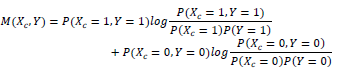
\includegraphics[width=5in]{img/fhr}
\caption{Formulae to calculate the transactions with mutual information}
\end{figure}where X and Y are random variables which determines the sampled transactions that belong to concept c and sampled transactions that belong to failure. We use the positive correlation part of the mutual information, ignoring the negative correlation events. The third step is, to exclude the noisy events i.e weakly discriminating events (for instance antivirus timeout) from the metric which has been obtained from the previous step.This is performed by using delta method. Transaction which satisfies the criteria are taken into consideration as the final signature of the events.The DMI is the weight of each term.The delta E which satisfies the given criteria are considered to be the signature of that issue.
2. Similar-issue retrieval 
Each issue is treated in the historical issue repository as one document, each signature as one term, and the corresponding delta mutual information (DMI) as the weight of each term. Each of the issues are treated as vectors. The similarity between two issue is determined by measuring the number of overlapping events between the two vectors.
3. Healing suggestion adaptation The Healing action is stored as verb + target + location, where verb is the healing action, target is the healing source and event is the new issue.

\begin{figure}[H]
\center
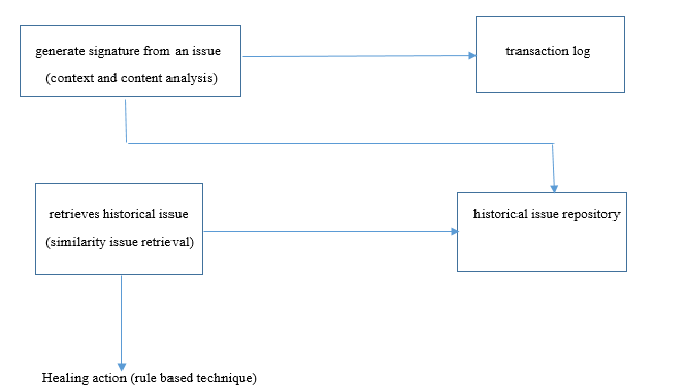
\includegraphics[width=5in]{img/historicalissue}
\caption{System architecture}
\end{figure}
\item[\textbf{Fault types}]
\item[\textbf{Failure types}] Performance failure
\item[\textbf{Input}] new issue
\item[\textbf{Recovery action}] Set of healing actions predefined in the historical repository.Healing actions are stored in the predicate$<verb + target + location>$
\item[\textbf{Advantages}] i) Reduces mean time to restore (MTTR) a failure, as the healing actions are priorly identified and restored in the historical repository.ii) Replaces manually healing action by an automated mining based approach. This is less time consuming and error prone.
\item[\textbf{Disadvantages}]i) the healing actions are predefined by the developers. In certain cases, if any fault occurs whose actions are not mentioned in the historical repository, that might cause system failure or crash.
\item[\textbf{Case study}] Deployed healing system in a production service, named ServiceX.
\end{compactitem}
\section{FUSION}\label{FUSION}
\begin{compactitem}
\item[\textbf{Title}]FUSION: A Framework for Engineering Self Tuning Self-Adaptive Software Systems
\item[\textbf{Author}]Ahmed Elkhodary,  Naeem  Esfahani, Sam Malek\item[\textbf{Reference}] 
\cite{elkhodary_fusion:_2012}

\item[\textbf{Year}] 2010

\item[\textbf{Application Domain}]Web services and QoS-based and AOP

\item[\textbf{Self-Healing steps}] Self-Healing steps   Self-healing steps involved the following:
(i) Detect 

(ii) Plan

(iii) Effect

\item[\textbf{Technical Approach}]
-Finite State Processes (FSP) and eXtensible Architecture Description Language (xADL)

\item[\textbf{Basic Idea}]  The study is on FUSION, which is feature oriented system model that learns the impact of feature selection and feature interaction for satisfying the system goals. From the learning, it adapts the system from failure recover and fulfils user defined goals. 

\item[\textbf{Summary of approach}] 
A self-adaptive software system is capable of modifying itself at run-time to achieve certain 
functional or QoS goals. However, development of such systems is challenging and requires foreseeing the changes in the environment, requirements and systems operational profile at design time. A framework FeatUre-oriented Self-adaptatION (FUSION) is developed which learns the 
impact of feature selection and features interaction on the systems goals. This knowledge efficiently helps adapting the system to meet user-defined goals.Fusion is based on two important parameters that are:

(i) Features-Based Adaptation

(ii) Goals

(i) Feature-based adaptation

The basic unit of adaptation is feature. Features represent the capability of the system. It can be a functional feature or non-functional feature. A functional feature can be print functions and a non-functional feature can be authentication properties. The feature in a system makes use of two kinds of relationships such as dependency and mutual. A dependency relationship indicates that a feature requires presence of another feature. Whereas mutual exclusion implies that if one of the features is in mutual group is enabled the others must be disabled. The enabled features are represented by 1 and disabled features are represented by 0. 

(ii) Goal

A goal represents the user’s functional or QoS objectives for a system. It includes two parameters

(i) Metric- measurable quantity obtained from running system (e.g. response time) 

(ii) Utility- function to represent user’s preference for a particular metric.

Fusion Model

Fusion model has been designed in two parts, Fusion Learning Cycle and Fusion Adaptation Cycle.

I. Fusion Learning Cycle
Fusion discovers the changing environment of the system through learning. Learning establishes the 
relationship between the features and metrics. Each relationship is represented as functions that 
calculate the features and their interactions, results a metric value. Each function takes a feature selection as input and produces an estimated gain/loss value for the metric as output. There are two activities that populate and fine tunes the knowledge.

a) Observe- Observe performs normalization of raw metric value that makes them suitable for 
learning. And also test the accuracy of learned functions with the currently observed 
collection of data. If the accuracy test fails, observe marks an indicator that either learning is 
incomplete or new patterns of behaviour has emerged.

b) Induce- From the collected information from Observe, Induce constructs functions that 
estimate the proper feature for a metric. 

i. Induce performs a significance test for determining the features that have significant 
impact on the metric. This test helps in reducing the number of independent variables 
that are considered for metric computation.

ii. After the normalization of data and extraction of features with significance, relationships are derived.

II. Fusion Adaptation Cycle

From the learned knowledge the system is adapted in this step with the DETECT, PLAN and EFFECT. A major principle for adaptation strategy is - “If the system works (i.e., satisfies the user), do not change it; when it breaks, find the best fix for only the broken part.” 

a. Detect- The detect determines the system goal violation. This is done by monitoring the utility 
functions. The utility function returns zero to indicate the violation of goals when metric 
value are unacceptable. It returns a positive value to indicate users preference for improvement when metrics satisfy. After the detection for goal violation is done the system initiates adaptation cycle.

b. Plan- The Plan eliminates all the features having no significant impact on goal. These affected features are known as Shared Features. These shared features represent the adaptation 
parameters. These features may also affect other goals, known as Conflicting Goals. To detect 
the conflicts, the knowledge base is used by back-tracking the learned relationships. FUSION 
generates an optimization problem with objective to find a selection of Shared Features that 
maximizes the system’s overall utility for the Conflicting Goals.

c. Effect-Once an optimal feature selection is determined, the Effect activity is initiated to make the system transition from the current feature selection to the new one. From three given paths such as enable, disable and swap mutually exclusive features, effect chooses path for new 
feature selection.
\item[\textbf{Fault Types}](i) System Perfomance
 
\item[\textbf{Failure Types}]
(i) Normal Traffic

(ii) Varying Traffic

(iii) Index Failure 

(iv) Randomized DoS Traffic
\item[\textbf{Input data}] 

(i)
\item[\textbf{Recovery actions}]
FUSION minimizes frequent adaptation of the system for the same problem. Instead of simply satisfying the violated goals, FUSION finds a near optimal solution that is less likely to be broken due to fluctuations in the system.

\item[\textbf{Advantages}] 

(i) A learning model is automatically induced from monitored data.

(ii) Automatic online fine-tuning of adaptation logic is done for unanticipated conditions.

(iii) It reduces the upfront effort required for constructing such systems.

(iv) FUSION is capable of learning run-time behaviours unforeseen at design-time.


\item[\textbf{Disadvantages}] 
(i) With DoS, the random nature of traffic makes FUSION to converge to an induced model. Hence FUSION cannot reach a better accuracy in DoS scenario. 

(ii) Due to inaccuracy of induced model, FUSION fails to predict the magnitude of the metrics.


\item[\textbf{Case study}] 
(i) Travel Reservation System

(ii) XTEAM

\end{compactitem}
